\begin{frame}{Thoughts}
    \begin{block}{Input}
        \begin{itemize}
            \item Different variable set $\rightarrow$ different problem topology
            \item Concatenate layers as input $\rightarrow$ Combination of more information and final output
            \item Separate background from the adversary's input $\rightarrow$ remove possible bias
        \end{itemize}
    \end{block}
    %
    \begin{block}{General}
        \begin{itemize}
            \item Different analysis $\rightarrow$ Insight on the network's general inability
        \end{itemize}
    \end{block}
\end{frame}

\begin{frame}{Conclusions}
    \begin{block}{Optimisation of a combination of networks}
        \begin{itemize}
            \item Classifier and adversary need to be optimised together rather than separately
        \end{itemize}
    \end{block}
    %
    \begin{block}{Input of the adversary}
        \begin{itemize}
            \item The complex architecture of the adversary is not justified by just inputting the classifier's output
        \end{itemize}
    \end{block}
    %
    \begin{block}{Strong dependency on the learning rate}
        \begin{itemize}
            \item Learning rate is the defining factor of the performance of the losses
            \item Presumably due to the fine topology around the minimum
        \end{itemize}
    \end{block}
\end{frame}

\begin{frame}{}
    \begin{figure}
        \centering
        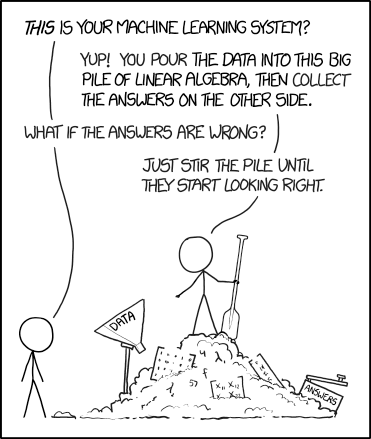
\includegraphics[width=0.4\textwidth]{xkcd}
        \caption{https://xkcd.com/1838/}
    \end{figure}
\end{frame}